\section{Datentypen}

Sie legen fest,

\begin{itemize}[itemsep=1pt, parsep=0pt]
    \item wie lang das Bitmuster an der zugehörigen Speicherstelle ist,
    \item und was dieses Bitmuster bedeutet.
\end{itemize}

\subsection{simple Ganzzahltypen}

\begin{itemize}[itemsep=1pt, parsep=0pt]
    \item \textbf{char} \newline immer 8 Bit (Als einziger Typ \textbf{IMMER} 1 Byte)
    \item \textbf{short} \newline für kleine ganzzahlige Werte (mind. 16 Bit)
    \item \textbf{int} \newline effizienteste Grösse für Prozessor (mind. 16 Bit)
    \item \textbf{long} \newline für grosse ganze werte (mind. 32 Bit)
    \item \textbf{long long} \newline für sehr grosse ganze werte (mind. 64 Bit)   
    \item \textbf{size\_t} \newline mindestens so gross wie die maximale Anzahl Adressen, nie negativ
\end{itemize}

Ganzzahltypen können \textbf{signed} (Vorzeichenbehaftet) oder \textbf{unsigned} sein. Wenn nicht definiert, meist signed ausser datentyp \textbf{char}, dieser ist nicht standardisiert.\newline
\textbf{Überlauf ist nicht definiertes Verhalten}\newline
Der \textbf{unsigned} Wertebereich befindet sich von 0 bis $2^n -1 $\newline
Der \textbf{signed} Wertebereich (Zweierkomplement)befindet sich von $-2^{n-1}$ bis $2^{n-1} -1 $\newline
(n = anzahl bits)

\subsection{Typedef Stdint.h}

Stdint stellt vordefinierte Typen zur Verfügung welche Plattform unabhängige feste Grössen haben. z.B. :
\begin{itemize}[itemsep=1pt, parsep=0pt]
    \item int8\_t = signed 8 Bit
    \item uint64\_t = unsigned 64 Bit
    \item .....
\end{itemize}
Allerdings sind diese auf dem Zielsystem möglicherweise nicht sehr effizient, da sie die native Busbreite über oder unterschreiten. Ein Int ist der effizienteste Datentyp.

\subsection{Gleitpunktzahl}

Gleitpunnktzahlen speichern Zahlen wissenschaftlicher Schreibweise. Dabei treten allerdings fast immer Rundungsfehler auf(\textbf{nie auf Gleichheit testen}) und brauchen viel Rechenleistung. Sie können aber auch Werte wie $\pm$ inf, $\pm$ 0, NaN(not a number) darstellen.\newline
Speicherzusammensetzung, Standardisierter float (IEEE 754): 
\begin{center}
    \begin{tabular}{|c|c|c|c|} \hline  
          & Sign  & Exponent & Mantisse \\ \hline  
        float & 1 & 8 & 23\\ \hline  
        double & 1 & 11 & 52 \\ \hline   
    \end{tabular}
\end{center}

Wenn eine Zahl mit einem Koma (z.B: 12.91) definiert wird, ist sie automatisch eine Gleitpunktzahl. Dieser Effekt kann verwendet werden, um bei eine Mathematischen Berechnung die Genauigkeit zu verbessern, wenn mit Ganzzahltypen gerechnet wird. Wenn eine Zahl implizit als Gleitpunktzahl (Möglichst am Anfang der Rechnung) definiert wird, wird implizit mit einer Gleitpunktzahl weiter gerechnet und am Schluss wieder zu einer Ganzzahl umgewandelt.

\subsection{Enum}

\subsubsection{Aufzählungstyp}

Mit einem Enum(im code immer klein schreiben) kann ein Aufzählungstyp erreicht werden für z.B. für state machines. Generelle Syntax:\newline
enum type-name \{item1 = value1, item2 = value2, …\};\newline
Die Value Deklaration kann ausgelassen werden. Der Compiler vergibt von 0 auf aufzählend automatisch Werte. Es kann strategisch eine Zahl dazwischen gesetzt werden um gewisse numerische Zahlen zu Erhalten.\newline
Wenn man ein Enum verwendet will, muss das Schlüsselwort "Enum" immer mitgeschrieben werden. Mit einer Typendeklaration kann das vereinfacht werden. 

\begin{lstlisting}[language = c]
enum groesse {LOW,MEDIUM,HIGH};//deklaration
enum groesse myVar;//Variable mit Typ enum
enum groesse myFunc();//Funktion mit rueckgabetyp Enum
\end{lstlisting}

\subsubsection{Ganzzahkonstanten}

Man kann per Enum auch Ganzzahlkonstanten definieren. Sie sind sicherer als ein \#define und erlauben auch das Definieren grössen eines Arrays. Definition:

\begin{lstlisting}[language = c]
enum{goodYear = 1291, badYear = 1848};
int arr[goodYear][badYear];//erlaubt, erstellt ein 2d Array
\end{lstlisting}

\subsection{Pointer}

Pointer sind Variablen welche eine Speicheradresse enthalten. Sie sind mindestens so gross, dass alle Speicheradressen definiert werden können.\newline
Wenn Pointer Referenziert(Operator : \&) werden, liest man die Adresse, auf die der Pointer zeigt.\newline
Wenn ein Pointer dereferenziert(Operator : *) wird, liest man den Wert, auf der gezeigt wird.\newline 
Pointer müssen auch den Variabeltyp, auf den sie Zeigen, definiert bekommen um das Bitmuster auf das sie zeigen Interpretieren zu können. Ausnahme davon sind die Voidpointer. Ihnen kann jeder Pointertyp übergeben werden. Diese dürfen aber \textbf{nicht} dereferenziert werden.\newline
Wenn ein Pointer nicht gebraucht wird, muss er "NULL" (nicht zwingend numerisch 0) gesetzt werden. Das Dereferenzieren eines NULLpointer  führt zu undefined behaviour.\newline

\begin{lstlisting}[language = c]
int* aPointer;//deklaration eines Pointers mit typ int
int* ptr = NULL;//NULL initialisierter Pointer
void* ptrb;//Deklaration eines Voidpointer
aPointer = &myInt;//aPointer zeigt nun auf die adresse von myInt
otherInt = *aPointer;//other uebernimmt den Wert von myInt
ptr = apointer;//Einem Voidpointer wird ein Pointer des Typs int* zugewisen
\end{lstlisting}

\subsubsection{Pointer Arithmetik}

\begin{itemize}[itemsep=1pt, parsep=0pt]
    \item Pointer unterschiedlicher Datentypen dürfen einander nicht zugewiesen werden (Schutzmechanismus)
    \item Einem Pointer eines bestimmten Typs dürfen Pointer dieses Typs oder void-Pointer zugewiesen werden
    \item Einem void-Pointer dürfen beliebige Pointer zugewiesen werden (nützlich, aber gefährlich)
\end{itemize}
Auf Pointer darf des weiteren addiert und subtrahiert werden. Ganze zahlen verschieben ihn dabei jeweils um ganze Elemente. Daher kann man nicht zwischen 2 Elemente Zeigen. Darum ist der Pointer Typ wichtig. Es ist keine Arithmetik auf einen Voidpointer möglich.\newline
Pointer darf man auch mit anderen Pointer vergleichen(==, !=,...).

\subsubsection{Memorymap}

Eine Memorymap wird verwendet, um den Zustand von Pointer und Variablen zu signalisieren. Das folgende Beispiel zeigt den Zustand von der Deklaration oben.\newline
\begin{center}
    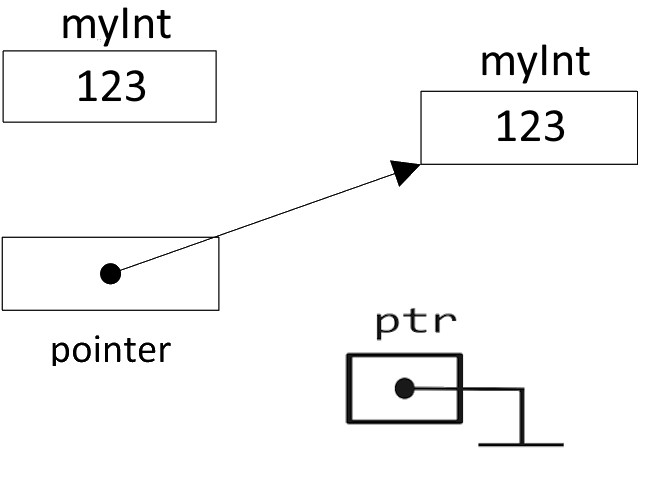
\includegraphics[width=.5\columnwidth]{Pictures/Pointer_memory_map.png}
\end{center}

\subsection{Deklarieren}

Generelle Syntax : \textless Datentyp \textgreater \textless Variablenname\textgreater;\newline
Erlaubte Zeichen sind Buchstaben, Ziffern und Underscore(\_). Eine Zahl darf nicht zu beginn stehen. Umlaute sind nicht erlaubt. Variablennamen sind \textbf{case sensitive!}\newline
Beispiele:

\begin{lstlisting}[language = c]
int ichbins; //korrekt
int 0ichbins; //falsch wegen der Zahl am Anfang
char ichbins1; //erlaubt da Zahl am Ende
double schwarz = 9.9; //mit Initialisierung
char eins, zwei, drei = 'a'; // mehrere Variablen werden initialisiert aber nur "drei" wird mit 'a' initialisiert 
\end{lstlisting}

Es gibt Namen, die nicht erlaubt sind, da sie vom C Standard reserviert sind. Diese sind:\newline

\begin{center}
    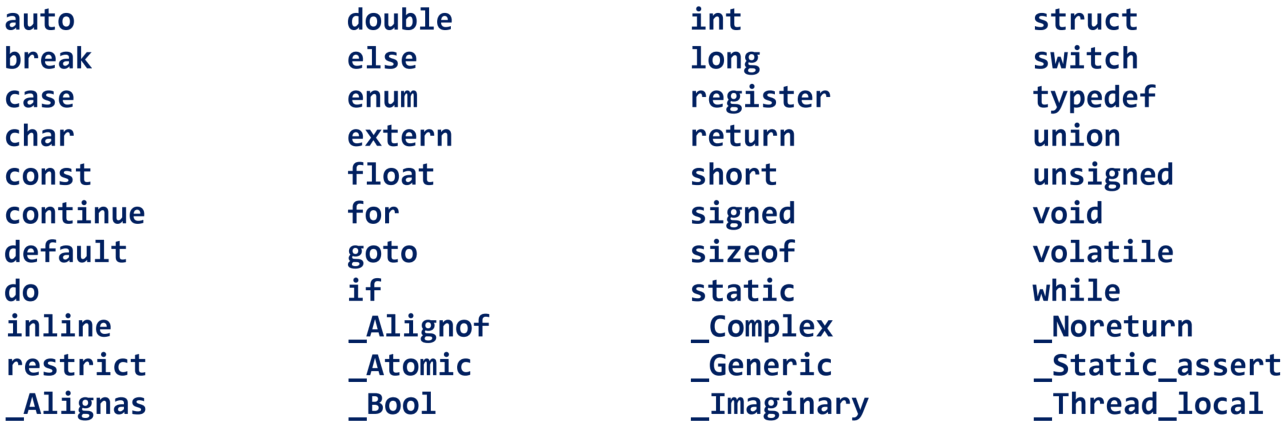
\includegraphics[width=1\columnwidth]{Pictures/illegal_variable_names.png}    
\end{center}

\subsection{Umwandeln}

Es gibt die implizite und explizite Umwandlung. Implizit erledigt der Compiler da er selbst ein missmatch von Typen erkennt $\rightarrow$ schlecht da es eine Warnung erzeugt.\newline
Explizit wird durch Schreiben des Typs neben der umzuwandelnden Zahl erreicht.

\begin{lstlisting}[language = c]
float flZahl = 41.7; //implizit: eine Kommazahl ohne f am Ende hat Typ double
int x = (int)flZahl; //explizit: x hat den Wert 41, Nachkommastellen werden abgeschnitten!
\end{lstlisting}

\subsection{Scope}

\begin{itemize}[itemsep=1pt, parsep=0pt]
    \item \textbf{global} \newline nicht in eine Funktion deklariert, 0 initialisiert, Laufzeit des Programms, immer sichtbar
    \item \textbf{lokal} \newline in Funktion deklariert, nicht initialisiert, Laufzeit der Funktion, nur in der Funktion Sichtbar, auch wenn eine neue Funktion aufgerufen wird.
    \item \textbf{static} variablen sind dabei eine Ausnahme(siehe Static$\rightarrow$ Typ-attribute).
\end{itemize}

\subsection{Arrays}

Ein Array bietet eine kompakte Zusammenfassung von mehreren Variablen des gleichen Basistyps. Arrays beginnen immer bei 0 und sind so lang wie definiert bei der Deklarierung. 
\begin{lstlisting}[language = c]
float messDat[12];//Ein Array fom typ float mit 12(0-11) Elementen wird deklariert
char text[groesse];//Ein Array fom typ char wird mit der konstanten "groesse" initialisiert 
messDat[20] = 12 //fuehrt zu undefined behaviour. Es wird ausserhalb des Arrays '12' geschrieben. Es kann irgendeine Speicherstelle ueberschriben werden.
\end{lstlisting}

\subsubsection{Initialisierung}

Man kann ein Array entweder komplett oder gar nicht initialisieren.

\begin{lstlisting}[language = c]
int a[4] = {1,2,9,1};//vollstaendige initialisierung
int b[4] = {6,9};// b[2],b[3] werden mit 0 initialisiert
int c[4] = {};//alle Elemente werden mit 0 initialisiert
int d[] = {1,2,9,1};//die groesse wird vom Compiler festgelegt
\end{lstlisting}

\subsubsection{Char Arrays}

Mit Char Arrays werden Zeichenketten realisiert. Char Arrays müssen immer NULL('\textbackslash 0') terminiert werden, wenn mit diesen Standardfunktionen zur Char Array Verarbeitung verwendet werden. Die Nullterminierung wird verwendet, um zu wissen wann die Zeichenkette fertig ist.

\begin{lstlisting}[language = c]
char name[15] = {77, 101, 106, 101, 114, 0};//numerische werte entsprechen der Ascii definition
char name[15] = {'M', 'e', 'i', 'e', 'r', '\0'};//einzelne chars
char name[15] = "Meier"; // bevorzugte Variante, enthaelt automatisch das Nullzeichen!
\end{lstlisting}

\subsubsection{Memorymap}

Das Format der Memorymap für Arrays sieht folgendermassen aus:\newline

\begin{tabular}{|c|c|c|c|c|}
\hline
Wert 0&Wert 1& Wert 2& Wert 3&Wert 4\\ \hline
\end{tabular}

Unter den jeweiligen Werten muss die Element Nummer Stehen.

\subsubsection{Handhabung von Arrays}

Arrays können nicht direkt miteinander verglichen werden, in Funktionen direkt übergeben werden oder direkt auf ein anderes überspielt werden (memcpy kann verwendet werden).\newline
Bei einem Funktionsaufruf wird ein Pointer auf das erste Element des Arrays übergeben.

\subsubsection{Mehrdimensionale Arrays}

Mehrdimensionale Arrays können so verstanden werden das ein Array Element wieder ein ganzes Array enthaltet.\newline
Bei einem 2D Array kann man sich eine Matrix vorgestellt wobei beim Aufruf [Zeile][Spalte] mitgegeben werden.\newline
Definition eines mehrdimensionalen Arrays:\newline
\noindent
\begin{minipage}{0.5\columnwidth}
\begin{lstlisting}[language = c]
int alpha[3][4] = {
{1, 2, 3, 4},
{5, 6, 7, 8},
{9, 0, 1, 2}};
\end{lstlisting}
\end{minipage}
\begin{minipage}{0.5\columnwidth}
\begin{tabular}{|c|c|c|c|}
\hline
1 & 2 & 3 & 4 \\ \hline
5 & 6 & 7 & 8 \\ \hline
9 & 0 & 1 & 2 \\ \hline
\end{tabular}
\end{minipage}

Ebenso könnte man alpha so initialisieren:

\begin{lstlisting}[language = c]
int alpha[3][4] = {1, 3, 5, 7, 2, 4, 6, 8, 3, 5, 7, 9};
\end{lstlisting}

\subsection{Pointer und Arrays}

Pointer und Arrays können ähnlich verwendet werden. In aufgerufenen Funktionen kann mit einem Pointer sowie mit einem Array weitergearbeitet werden. 

\begin{lstlisting}[language = c]
int* iptr;
int iarr[4] = {1,8,4,8};
iptr = iarr;// ein Array wird implizit zu einem Pointer des Basis-Typs gewandelt
iptr = &iarr[0];//macht dasselbe
iptr = &iarr;// Achtung: macht nicht dasselbe! Fuehrt zu einem Compiler-Fehler!

iarr[3] = 12;
iptr[3] = 12;
*(iptr+3) = 12;//macht 3-mal dasselbe
\end{lstlisting}

\subsubsection{Char Array}

Eine String Definition kann auch so erfolgen:
\begin{lstlisting}[language = c]
char str[] = "Ich gehoere ins printf";
char* str = "Ich gehoere ins printf";
printf("%s\n", str);
\end{lstlisting}

\subsection{Typ-attribute}

\subsubsection{const}

Das Attribut const (vor dem Variablentyp geschrieben) markiert eine Variable als read only für den Quellcode, die Hardware kann aber dennoch den Wert verändern.\newline
Ein Const Array besteht nur aus konstanten.\newline
Für ein konstanten Pointer muss const nach dem * stehen. Sonst ist nur der Wert auf den der Pointer zeigt read only. 

\begin{lstlisting}[language = c]
const char* text;//pointer auf einen konstanten text
const char* const text;//konstanter pointer auf einen konstanten text
"text"//string literal -> konstanter text
\end{lstlisting}

Um sicherzugehen was wirklich konstant ist kann die Definition von rechts nach links gelesen werden. Was links neben einem const steht ist wirklich const.\newline

In Funktionsköpfen lohnt es sich const als Sicherheit einzubauen, so das nicht versehentlich eine variable geschrieben wird.
\begin{lstlisting}[language = c]
void foo(const int* const ptr);//der int wert und Pointer kann nicht mehr versehentlich veraendert werden.
\end{lstlisting}

\subsubsection{Volatile}

Volatile signalisiert dem Compiler das sich die Variable auch ausserhalb der normalen Programmausführung ändern kann. Einsatz bei Hardware naher Programmierung und multithreading.

\subsubsection{static}

Static kann eine Variabel und eine Funktion sein, diese haben aber jeweils verschiedene Bedeutungen:
\begin{itemize}
    \item Globale Variabel oder Funktion:\newline
    Sie sind nur in der Compile Unit gültig in der sie definiert sind.
    \item lokale Variabel:\newline
    haben dieselbe \textbf{Lebensdauer wie eine Globale Variabel}, Sichtbarkeit auf Funktionsblock beschränkt und mit 0 oder einer konstanten  einmalig initialisiert. 
\end{itemize}

\subsection{Structs}

Mittels Struct kann man verschiedene Datentypen zu einem Typ zusammenführen. Auch Structs kann man in einen anderen Struct verwenden.\newline

\noindent
\begin{minipage}{0.5\columnwidth}
Definition:
\begin{lstlisting}[language = c]
struct structname
{
    typ1 name1;
    typ2 name2;
    typ3 name3;
    typn namen;
}
\end{lstlisting}
\end{minipage}
\begin{minipage}{0.5\columnwidth}
bsp:
\begin{lstlisting}[language = c]
struct adresse
{
    int postleitzahl;
    char strasse[20];
    int hausnummer;
    char land[3];
}
\end{lstlisting}
\end{minipage}

\subsubsection{Beispiel mit Pointer}

Das Beispiel verwendet Deklarationen von oben

\begin{lstlisting}[language = c]
int main()
{
    struct adresse home = {8640,"teststr",42,"CH"};
    printf("%d %s %s",home.postleitzahl,home.strasse,home.land);//direkter zugriff
    //der "." Operator wird verwendet fuer Elementzugriff
    
    struct adresse* ptr = &home;
    printf("%d %s %s",(*ptr).postleitzahl,ptr->strasse,ptr->land);//pointer zugriff
    //der "->" operator ist zu bevorzugen
}
\end{lstlisting}

\subsubsection{Grösse}

Die Grösse eines Struct ist nicht immer die Summe aller Typen. Aufgrund von Hardwarelimitationen (Alignment) können padding bytes in der Struct eingesetzt werden welche einfach leer sind. Daher kann man die wirkliche Grösse nur durch sizeof herausfinden.

\subsubsection{Funktionen}

Funktionsaufrufparameter und Funktionsreturns können Structs sein. Allerdings ist dies nicht effizient und eine Übergabe des Pointers wäre besser da in diesem Fall auch Arrays direkt üergeben werden.

\subsection{Union}

Unions haben eine identische Syntax wie Structs, allerdings teilen \textbf{alle} Elemente den \textbf{selben} Speicherbereich. Man kann es verwenden, um z.B. einfacher an die einzelnen Bytes einer IpV4 Adresse zu kommen.
\begin{lstlisting}[language = c]
union IPv4Address
{
    uint8_t addressByte[4];
    uint32_t address;
};//Die Ipv4 Adresse kann nun entweder als ganzer Block gelesen werden oder die 4 bytes seperat. 
\end{lstlisting}

\subsection{typedef}

Man kann sich auch eigene Typennamen erstellen mit typedef.\newline
syntax : typedef \textless Typ \textgreater \textless Name des neuen typ\textgreater\newline
stdint.h verwendet dies. Auch sehr nützlich um das Schlüsselwort Enum/Struct zu sparen. 
\begin{lstlisting}[language = c]
enum state {...};
typedef enum state State_t;
//jetzt kann ich State_t schreiben anstatt enum state.

typedef enum{...} State_T;
//Macht dasselbe aber kuerzer
\end{lstlisting}